% ============================================================
% IPW3 -- Participants
% ============================================================

\begin{frame}{\small IPW3 -- Onera M6 Participants}
\scriptsize

% IPW3 participant colors
\definecolor{p001}{HTML}{2CA02C}
\definecolor{p002}{HTML}{17BECF}
\definecolor{p003}{HTML}{00695C}
\definecolor{p004}{HTML}{BCBD22}
\definecolor{p006}{HTML}{9467BD}
\definecolor{p007}{HTML}{1F77B4}
\definecolor{p008}{HTML}{D62728}
\definecolor{p009}{HTML}{A5006A}
\definecolor{p010}{HTML}{0047FF}
\definecolor{p013}{HTML}{637939}
\definecolor{p014}{HTML}{E377C2}
\definecolor{p015}{HTML}{393B79}
\definecolor{p019}{HTML}{E6550D}
\definecolor{p020}{HTML}{843C39}

\centering

\renewcommand{\arraystretch}{1.20}
\setlength{\tabcolsep}{8pt}

\begin{tabular}{ccc}
\toprule
\textbf{ID} &
\textbf{Participant / Organization} &
\textbf{Color} \\
\midrule

001 & CIRA                   & \textcolor{p001}{\rule{1.5cm}{1.5pt}} \\
002 & AeroTex                & \textcolor{p002}{\rule{1.5cm}{1.5pt}} \\
003 & NRC                    & \textcolor{p003}{\rule{1.5cm}{1.5pt}} \\
004 & ONERA                  & \textcolor{p004}{\rule{1.5cm}{1.5pt}} \\
007 & Polytechnique Montréal & \textcolor{p007}{\rule{1.5cm}{1.5pt}} \\
010 & NASA                   & \textcolor{p010}{\rule{1.5cm}{1.5pt}} \\
015 & NIAR                   & \textcolor{p015}{\rule{1.5cm}{1.5pt}} \\
019 & Synopsys               & \textcolor{p019}{\rule{1.5cm}{1.5pt}} \\

\bottomrule
\end{tabular}

\end{frame}

\section[Case \& Submissions]{\textbf{Case Conditions \& Submission Summary}}

% ============================================================
% ONERA M6 -- Geometry and Aerodynamic Conditions
% ============================================================

\begin{frame}{\small Geometry and Aerodynamic Conditions}
\scriptsize

\begin{columns}[T,onlytextwidth]

%------------------------------------------------
\begin{column}{0.43\textwidth}
\centering
\begin{figure}
    \centering
    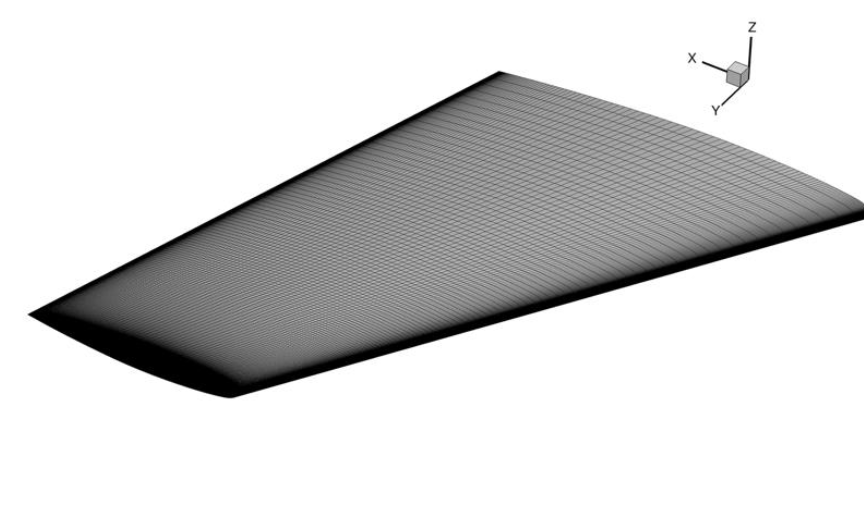
\includegraphics[height=0.6\textheight]{FIGURES_CONDITIONS/ONERA_M6_GEOMETRY_VIEW.png}
\end{figure}

\vspace{-0.15cm}

\centering
\textbf{ONERA M6 L1 Surface Mesh}

\end{column}

%------------------------------------------------
\begin{column}{0.53\textwidth}
\centering
\textbf{Geometry}

\vspace{0.15cm}

\begin{tabular}{lc}
\toprule
\textbf{Parameter} & \textbf{Value} \\
\midrule
Wing & ONERA M6 \\
Root chord [m] & $1.0$ \\
Semi-span [m] & $1.4760$ \\
Mean aerodynamic chord [m] & $0.801673$ \\
Reference area [m$^2$] & $1.1532$ \\
Angle of attack, $\alpha$ [$^\circ$] & $2.0$ \\
\bottomrule
\end{tabular}

\vspace{0.35cm}

\textbf{Aerodynamic Conditions}

\vspace{0.15cm}

\begin{tabular}{lc}
\toprule
\textbf{Parameter} & \textbf{Value} \\
\midrule
$M_\infty$ [-] & $0.40$ \\
$U_\infty$ [m/s] & $131.064$ \\
$T_\infty$ [K] & $267.15$ \\
$\rho_\infty$ [kg/m$^3$] & $0.68301$ \\
$Re_c$ [-] & $4.2558\times10^6$ \\
\bottomrule
\end{tabular}

\vspace{0.35cm}

\textbf{Quantities of Interest}

\vspace{-0.35cm}

\[
C_L,\qquad C_D,\qquad C_M,\qquad C_p
\]

\end{column}

\end{columns}

\end{frame}


% ============================================================
% ONERA M6 -- Icing Conditions
% ============================================================

\begin{frame}[shrink]{\small Icing Conditions}
\scriptsize

\begin{columns}[T,onlytextwidth]

%------------------------------------------------
\begin{column}{0.43\textwidth}
\centering
\begin{figure}
    \centering
    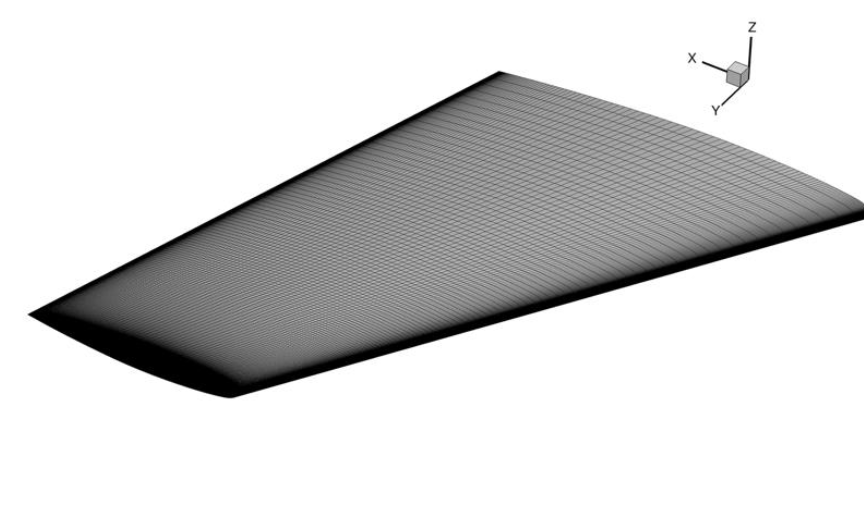
\includegraphics[height=0.6\textheight]{FIGURES_CONDITIONS/ONERA_M6_GEOMETRY_VIEW.png}
\end{figure}

\vspace{-1.0cm}

\textbf{ONERA M6 L1 Surface Mesh}

\vspace{0.20cm}

\centering
\begin{tabular}{lc}
\toprule
\textbf{Grid} & \textbf{Nodes} \\
\midrule
L1 & $60.78$ M \\
L2 & $7.63$ M \\
L3 & $0.960$ M \\
L4 & $0.122$ M \\
\bottomrule
\end{tabular}

\end{column}

%------------------------------------------------
\begin{column}{0.53\textwidth}
\centering
\textbf{Icing Conditions}

\vspace{0.15cm}

\begin{tabular}{lc}
\toprule
\textbf{Parameter} & \textbf{Value} \\
\midrule
$T_\infty$ [K]          & $267.15$ \\
$T_0$ [K]               & $275.7$ \\
$M_\infty$              & $0.40$ \\
$U_\infty$ [m/s]        & $131.064$ \\
LWC [g/m$^3$]           & $0.51$ \\
MVD [$\mu$m]            & $20$ \\
Exposure time [s]       & $1350$ \\
\bottomrule
\end{tabular}

\vspace{0.30cm}

\textbf{Droplet Distribution} : 1, 3, 7 $\&$ 15 bin distributions are considered

\vspace{0.25cm}

\begin{block}{\scriptsize Common Modeling Parameters}

A dimensional roughness of \textbf{$k_s=1.0$ mm} is prescribed as the baseline, and a common ice density of \textbf{$\rho_{\mathrm{ice}}=680~\mathrm{kg/m^3}$} is used for the comparison.

\end{block}

\vspace{0.35cm}

\textbf{Quantities of Interest}

\vspace{-0.35cm}

\[
\beta,\quad HTC,\quad T_s,\quad FF,\quad
m_{\mathrm{water}},\quad m_{\mathrm{ice}},\quad
m_{\mathrm{evap}}
\]

\end{column}

\end{columns}

\end{frame}

% ============================================================
% ONERA M6 -- Modeling Choices
% ============================================================

\begin{frame}{\small ONERA M6 -- Modeling Choices Across Submissions}
\scriptsize

\centering

\renewcommand{\arraystretch}{1.40}
\setlength{\tabcolsep}{2.2pt}

\begin{tabular}{c|ccccc}
\toprule
\textbf{Model / Method}
& \textbf{001}
& \textbf{002}
& \textbf{004}
& \textbf{007}
& \textbf{019} \\
\midrule

\textbf{Turbulence}
& $k$--$\omega$ TNT
& $k$--$\omega$ SST
& $k$--$\omega$ SST
& SA
& $k$--$\omega$ SST \\

\textbf{Droplet formulation}
& Eul.
& Lag.
& Eul.
& Eul.
& Eul. \\

\textbf{HTC method}
& --
& BL Int.
& $T_{rec}$
& $T_{rec}$
& -- \\

\textbf{Thermodynamics}
& Mess.
& Mess.
& Mess.
& Mess.
& SWIM+ \\

\textbf{Geometry evolution}
& Lag./IB
& Interp.
& --
& Lag.
& Lag./remesh \\

\textbf{No. of shots}
& $1$ / Multi
& $1$
& $1$
& $1$
& Multi \\

\bottomrule
\end{tabular}%


\vspace{0.12cm}

\begin{minipage}{0.98\textwidth}
\tiny
\textit{
Eul. = Eulerian;
Lag. = Lagrangian;
SA = Spalart--Allmaras;
BL Int. = boundary-layer integral;
$T_{rec}$ = recovery temperature;
Mess. = Messinger;
SWIM = shallow-water icing model;
IB = immersed boundary;
ALE = arbitrary Lagrangian--Eulerian;
Interp. = interpolation;
disp. = displacement;
Multi = multilayer/multishot;
-- = not reported.
}
\end{minipage}

\vspace{0.10cm}

\begin{block}{\scriptsize Overall Trends}
\begin{itemize}
    \item $k$--$\omega$ SST and Eulerian droplet formulations are the predominant choices among the disclosed submissions.
    \item Thermodynamic modeling is predominantly Messinger-based, while geometry-evolution methods are more diverse.
    \item Both single-shot and multishot strategies are represented.
\end{itemize}
\end{block}

\end{frame}

% ============================================================
% ONERA M6 -- Data Received
% ============================================================

\begin{frame}{\small ONERA M6 -- Summary of Data Received}
\scriptsize

\centering

\renewcommand{\arraystretch}{1.15}
\setlength{\tabcolsep}{3.5pt}

\begin{tabular}{c|cccc|cccc|cccc|cccc}
\toprule
&
\multicolumn{4}{c|}{\textbf{L1}} &
\multicolumn{4}{c|}{\textbf{L2}} &
\multicolumn{4}{c|}{\textbf{L3}} &
\multicolumn{4}{c}{\textbf{L4}} \\

\textbf{ID}
& 1 & 3 & 7 & 15
& 1 & 3 & 7 & 15
& 1 & 3 & 7 & 15
& 1 & 3 & 7 & 15 \\
\midrule

001 & \checkmark&&& & \checkmark&\checkmark&\checkmark&\checkmark & \checkmark&\checkmark&\checkmark&\checkmark & \checkmark&\checkmark&\checkmark&\checkmark \\

002 & \checkmark&\checkmark&\checkmark&\checkmark & \checkmark&\checkmark&\checkmark&\checkmark & \checkmark&\checkmark&\checkmark&\checkmark & \checkmark&\checkmark&\checkmark&\checkmark \\

003 & &&& & \multicolumn{4}{c|}{$*$} & \multicolumn{4}{c|}{$*$} & \multicolumn{4}{c}{$*$} \\

004 & \checkmark&\checkmark&\checkmark&\checkmark & \checkmark&\checkmark&\checkmark&\checkmark & \checkmark&\checkmark&\checkmark&\checkmark & \checkmark&\checkmark&\checkmark&\checkmark \\

007 & \checkmark&\checkmark&\checkmark&\checkmark & \checkmark&\checkmark&\checkmark&\checkmark & \checkmark&\checkmark&\checkmark&\checkmark & \checkmark&\checkmark&\checkmark&\checkmark \\

010 & \checkmark&\checkmark&\checkmark&\checkmark & \checkmark&\checkmark&\checkmark&\checkmark & \checkmark&\checkmark&\checkmark&\checkmark & \checkmark&\checkmark&\checkmark&\checkmark \\

015 & \checkmark&\checkmark&\checkmark&\checkmark & \checkmark&\checkmark&\checkmark&\checkmark & \checkmark&\checkmark&\checkmark&\checkmark & \checkmark&\checkmark&\checkmark&\checkmark \\

019 & \checkmark&\checkmark&\checkmark&\checkmark & \checkmark&\checkmark&\checkmark&\checkmark & \checkmark&\checkmark&\checkmark&\checkmark & \checkmark&\checkmark&\checkmark&\checkmark \\

\midrule
\textbf{Total}
& \textbf{7} & \textbf{6} & \textbf{6} & \textbf{6}
& \textbf{7} & \textbf{7} & \textbf{7} & \textbf{7}
& \textbf{7} & \textbf{7} & \textbf{7} & \textbf{7}
& \textbf{7} & \textbf{7} & \textbf{7} & \textbf{7} \\
\bottomrule
\bottomrule
\end{tabular}

\vspace{0.15cm}


\parbox{0.95\textwidth}{\scriptsize\raggedright
\centering
\checkmark: populated CutData received for the corresponding droplet-bin distribution.
\\
$*$: Excel results only, no CutData slices.
}

\end{frame}